\subsection{Gauss-Legendre積分}
\begin{NoteBox}{Gauss-Legendre積分の二次元への拡張}{Integral-Gauss-Legendre-2D}
  \begin{equation}
    \label{Eq:Gauss-Legendre-2D}
    \int_{-1}^{+1}\int_{-1}^{+1} f\pab{\xi, \eta}\odif{\xi}\odif{\eta} \approx \sum_{i=1}^{N_\mathrm{sample}}\sum_{j=1}^{N_\mathrm{sample}}w_i w_j f\pab{\xi_i, \eta_j}
  \end{equation}
  \small
  $N_\mathrm{sample}$:サンプル点の数,$w_i$:重み,$\xi_i$,$\eta_i$:サンプル点
\end{NoteBox}
\eqref{Eq:Gauss-Legendre-2D}式を用いたときの積分の概念図を示す.このとき,サンプル点は2点とする.
\begin{figure}[H]
  \centering
  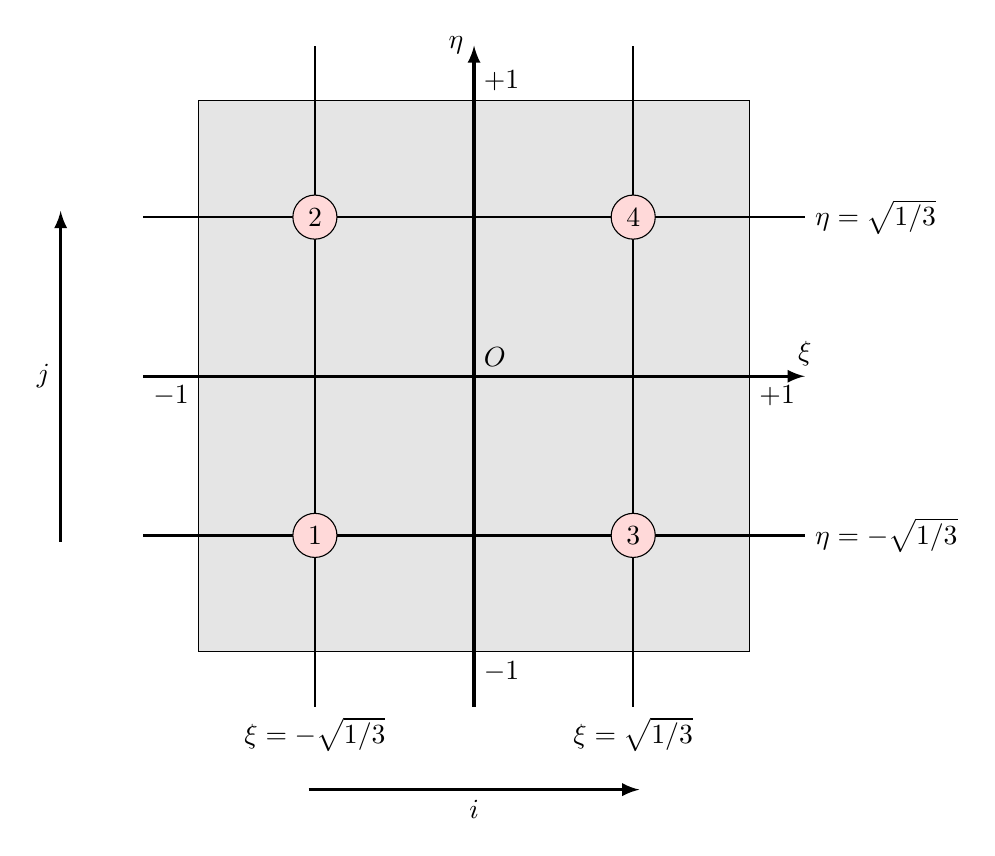
\begin{tikzpicture}[scale=3.5]
    \coordinate (p1) at (-1,-1);
    \coordinate (p2) at (1,-1);
    \coordinate (p3) at (1,1);
    \coordinate (p4) at (-1,1);
    \coordinate (S1) at (-0.57735,-0.57735);
    \coordinate (S2) at (-0.57735, 0.57735);
    \coordinate (S3) at ( 0.57735,-0.57735);
    \coordinate (S4) at ( 0.57735, 0.57735);

    \draw[fill=black!10!white] (p1)--node[midway, below right]{$-1$}(p2)--node[midway, below right]{$+1$}(p3)--node[midway, above right]{$+1$}(p4)--cycle node[midway, below left]{$-1$};
    \coordinate[label=above right:$O$] (O) at (0,0);
    %axis
    \draw[-{latex}, line width=0.4mm] (-1.2,0) -- (1.2,0) node[above]{$\xi$};
    \draw[-{latex}, line width=0.4mm] (0,-1.2) -- (0,1.2) node[left]{$\eta$};

    \draw[-{latex}, line width=0.4mm] (-0.6,-1.5) --node[midway, below]{$i$} (0.6,-1.5);
    \draw[-{latex}, line width=0.4mm] (-1.5,-0.6) --node[midway, left]{$j$} (-1.5,0.6);

    \draw[-, line width=0.3mm] (-1.2, 0.57735) -- (1.2, 0.57735) node[right]{$\eta= \sqrt{1/3}$};
    \draw[-, line width=0.3mm] (-1.2,-0.57735) -- (1.2,-0.57735) node[right]{$\eta=-\sqrt{1/3}$};
    \draw[-, line width=0.3mm] (-0.57735,-1.2) node[below]{$\xi=-\sqrt{1/3}$} -- (-0.57735,1.2);
    \draw[-, line width=0.3mm] ( 0.57735,-1.2) node[below]{$\xi= \sqrt{1/3}$} -- ( 0.57735,1.2);

    \foreach \i in {1,2,3,4} {
      \draw[fill=pink!60!white] (S\i) node {\i} circle[radius=0.08];
    }
  \end{tikzpicture}
  \caption{Gauss-Legendre積分のサンプル点を2点とした場合の積分の概念図}
\end{figure}
サンプル点は増やすことができる.サンプル点数に応じた,重みとサンプル点を表に示す.
\begin{longtable}{ccc}
  % \centering
  \caption{Gauss-Legendre積分のサンプル点数に応じた重みとサンプル点}\\
  % \begin{tabular}
    \hline
    サンプル点数:$N_\mathrm{sample}$ & サンプル点:$\xi_i$,$\eta_i$ & 重み:$w_i$,$w_j$\\
    \hline
    $1$ & $0$ & $2$\\
    \hline
    &&\\[-6mm]
    $2$ & $\pm\sqrt{\dfrac{1}{3}}$ & $1$\\[4mm]
    \hline
    &&\\[-6mm]
    $3$ & $0$ & $\dfrac{8}{9}$\\[4mm]
     & $\pm\sqrt{\dfrac{3}{5}}$ & $\dfrac{5}{9}$\\[4mm]
    \hline
    &&\\[-6mm]
    $4$ & $\pm\sqrt{\dfrac{3}{7}-\dfrac{2}{7}\sqrt{\dfrac{6}{5}}}$ & $\dfrac{18+\sqrt{30}}{36}$\\[4mm]
     & $\pm\sqrt{\dfrac{3}{7}+\dfrac{2}{7}\sqrt{\dfrac{6}{5}}}$ & $\dfrac{18-\sqrt{30}}{36}$\\[4mm]
    \hline
    &&\\[-6mm]
    $5$ & $0$ & $\dfrac{128}{225}$\\[4mm]
     & $\pm\dfrac{1}{3}\sqrt{5-2\sqrt{\dfrac{10}{7}}}$ & $\dfrac{322+13\sqrt{70}}{900}$\\[4mm]
     & $\pm\dfrac{1}{3}\sqrt{5+2\sqrt{\dfrac{10}{7}}}$ & $\dfrac{322-13\sqrt{70}}{900}$\\[4mm]
    \hline
  % \end{tabular}
\end{longtable}

何個か例題を解いて,精度を見てみることとする.

\begin{ExampleBox}{ガウス求積法}{GL-Integral-Example}
  Gauss-Legendre積分を用いて次の積分を求め,解析解と比較せよ.
  \begin{enumerate}[label=(\arabic*)]
    \item
    \begin{equation*}
      \int_{-1}^{+1}\int_{-1}^{+1} \pab{x^2 + y^2}\odif{x}\odif{y}
    \end{equation*}
    \item
    \begin{equation*}
      \int_{-1}^{+1}\int_{-1}^{+1} \pab{x^3 + y^3}\odif{x}\odif{y}
    \end{equation*}
    \item
    \begin{equation*}
      \int_{-1}^{+1}\int_{-1}^{+1} \exp\pab{-x^2 - y^2}\odif{x}\odif{y}
    \end{equation*}
    \item
    \begin{equation*}
      \int_{-1}^{+1}\int_{-1}^{+1} \pab{\sin x \cos y}\odif{x}\odif{y}
    \end{equation*}
  \end{enumerate}
\end{ExampleBox}
例題\ref{Exa:GL-Integral-Example}の解答を示す.

\begin{longtable}[c]{cS[table-format=1.8e-2] S[table-format=1.8e-2] S[table-format=1.8e-2] c}
  \caption{数値計算結果と解析解} \label{tab:results} \\

  \toprule
  & {$N_\mathrm{sample}$} & {結果} & {誤差} & {解析解} \\
  \midrule
  \endfirsthead

  \multicolumn{5}{c}%
  {{\bfseries 表 \thetable\  続き}} \\
  \toprule
  & {$N_\mathrm{sample}$} & {結果} & {誤差} & {解析解} \\
  \midrule
  \endhead

  \midrule
  \multicolumn{5}{r}{{続く}} \\
  \endfoot

  \bottomrule
  \endlastfoot

  \multirow{5}{*}{(1)} 
    & 1 & \SI{0.00000000E+00}{} & \SI{2.66666667E+00}{} & \multirow{5}{*}{\(\dfrac{8}{3}\)} \\
    & 2 & \SI{2.66666667E+00}{} & \SI{0.00000000E+00}{} &  \\
    & 3 & \SI{2.66666667E+00}{} & \SI{4.44089210E-16}{} &  \\
    & 4 & \SI{2.66666667E+00}{} & \SI{4.44089210E-16}{} &  \\
    & 5 & \SI{2.66666667E+00}{} & \SI{4.44089210E-16}{} &  \\
  \midrule
  \multirow{5}{*}{(2)} 
    & 1 & \SI{0.00000000E+00}{} & \SI{0.00000000E+00}{} & \multirow{5}{*}{\(0\)} \\
    & 2 & \SI{0.00000000E+00}{} & \SI{0.00000000E+00}{} &  \\
    & 3 & \SI{-5.55111512E-17}{} & \SI{5.55111512E-17}{} &  \\
    & 4 & \SI{2.77555756E-17}{} & \SI{2.77555756E-17}{} &  \\
    & 5 & \SI{1.38777878E-17}{} & \SI{1.38777878E-17}{} &  \\
  \midrule
  \multirow{5}{*}{(3)} 
    & 1 & \SI{4.00000000E+00}{} & \SI{1.76901486E+00}{} & \multirow{5}{*}{\(\pi\,\mathrm{erf}(1)^2\)} \\
    & 2 & \SI{2.05366848E+00}{} & \SI{1.77316665E-01}{} &  \\
    & 3 & \SI{2.24604053E+00}{} & \SI{1.50553890E-02}{} &  \\
    & 4 & \SI{2.23004829E+00}{} & \SI{9.36846798E-04}{} &  \\
    & 5 & \SI{2.23103191E+00}{} & \SI{4.67666046E-05}{} &  \\
  \midrule
  \multirow{5}{*}{(4)} 
    & 1 & \SI{0.00000000E+00}{} & \SI{0.00000000E+00}{} & \multirow{5}{*}{\(0\)} \\
    & 2 & \SI{0.00000000E+00}{} & \SI{0.00000000E+00}{} &  \\
    & 3 & \SI{-2.77555756E-17}{} & \SI{2.77555756E-17}{} &  \\
    & 4 & \SI{1.38777878E-17}{} & \SI{1.38777878E-17}{} &  \\
    & 5 & \SI{0.00000000E+00}{} & \SI{0.00000000E+00}{} &  \\
\end{longtable}

\begin{figure}[H]
  \centering
  \subfigure[$f\pab{x,y}=x^2 + y^2$]{\includegraphics[width=0.45\textwidth]{Gauss_f1.png}}
  \subfigure[$f\pab{x,y}=x^3 + y^3$]{\includegraphics[width=0.45\textwidth]{Gauss_f2.png}} \\
  \subfigure[$f\pab{x,y}=\exp\pab{-x^2 - y^2}$]{\includegraphics[width=0.45\textwidth]{Gauss_f3.png}}
  \subfigure[$f\pab{x,y}=\sin x \cos y$]{\includegraphics[width=0.45\textwidth]{Gauss_f4.png}}
  \caption{例題1の関数の概形}
\end{figure}
ただし,基底関数の積分においては基本的には要素が持っている次数+1のサンプル点数を用いることが多い.
また,必ずしもGauss-Legendre積分による積分が精度が保証されているわけではないので注意されたい.要素次元を増やすことよりも,サンプル点の座標をうまく調整することで精度を向上させることができる.例えば,2点での積分を行う場合には,サンプル点を$\xi_i=\pm 0.8165$とすることで,精度を向上させることができる.